\section{Thermal-Hydraulics System Code \glsentryshort{trace}}\label{sec:reflood_trace}

\gls[hyper=false]{trace} is the best-estimate system \gls[hyper=false]{th} code developed by the \gls[hyper=false]{usnrc} 
as a tool for light water reactor transient analysis during normal and accident scenarios.
Its development is an on-going effort 
to modernize into a single software package all previous \gls[hyper=false]{usnrc} \gls[hyper=false]{th} codes
that were developed separately for specific reactor types and/or applications.
This ultimately would make the code more versatile for end users and more efficient to maintain for the developer.

\subsection{Thermal-hydraulics System Code}\label{sub:th_system_code}

% What is system code
Thermal-hydraulics system code is a computer code used to analyze the thermal-hydraulics behavior of \glspl[hyper=false]{npp} \cite{Roth2014}.
\marginpar{thermal-hydraulics system code}
Its current usage ranges from safety analysis and licensing process of current reactor designs to qualification of a new reactor design \cite{Petruzzi2008, Petruzzi2016}.
To that end, the code is designed to be a comprehensive tool capable of simulating wide range of operating conditions, 
from normal operations, anticipated transients, to accident scenarios foreseen in nuclear power plant operation.

% Component-based system code
Nuclear reactor system is a complex system of numerous interconnected components, each serving distinct purpose, built with multiple engineered safety features.
During a transient, the system might exhibit complex behavior with important physical phenomena interacting at vastly different time scales ($10^{-1} \, [s]$ in a power excursion due to control rod ejection, $10^5 \, [s]$ for decay heat removal after successful reactor shutdown) and
length scales ($10^{-3} \, [mm]$ for boiling at sub-channel level, $10^3 \, [m]$ for coolant flow in the primary/secondary circuit).
Additionally, the engineered safety features are designed for some equipments (such as control rods, valves, pump, etc.) to perform safety-related action.
Such equipments, in turn, is controlled by a complex dynamical control system.
As such, system code has to take into account these different aspects to properly simulate the thermal-hydraulics behavior of nuclear power plants.
Indeed, com\-ponent-based codes, such as \gls[hyper=false]{trace}, approach the problem by representing each prominent component in nuclear reactor system separately.
On top of a two-phase fluid dynamics equation solver, system code includes models for steam separator, pump, heat exchanger, valve, pressurizer, and neutron-kinetics 
as well as comprehensive models for control system to mimic the signal monitoring and component action actuation systems in a \gls[hyper=false]{npp}.   
System thermal-hydraulics thus distinguishes itself by considering explicitly the geometry, materials, boundary conditions, various interconnecting components, and control systems that constitute an \gls[hyper=false]{npp} \cite{DAuria2012}.


% The essence of the problem tackled in thermal-hydraulics system code
However, it can be argued that the modeling of two-phase flow inside a heated channel remains a central part in nuclear thermal-hydraulics analysis 
\marginpar{basic thermal-hydraulics, two-phase flow in a heated channel}
which puts an emphasis in the correct prediction of cladding temperature evolution during different postulated scenarios. 
This is also supported by the fact that the majority of operating nuclear power plants is of \gls[hyper=false]{lwr} type, 
where two-phase flow can be expected to occur during its operation, both in normal operating and accident condition for \glspl[hyper=false]{bwr} and in accident condition for \glspl[hyper=false]{pwr}.
\begin{figure}[bth]
	\centering
	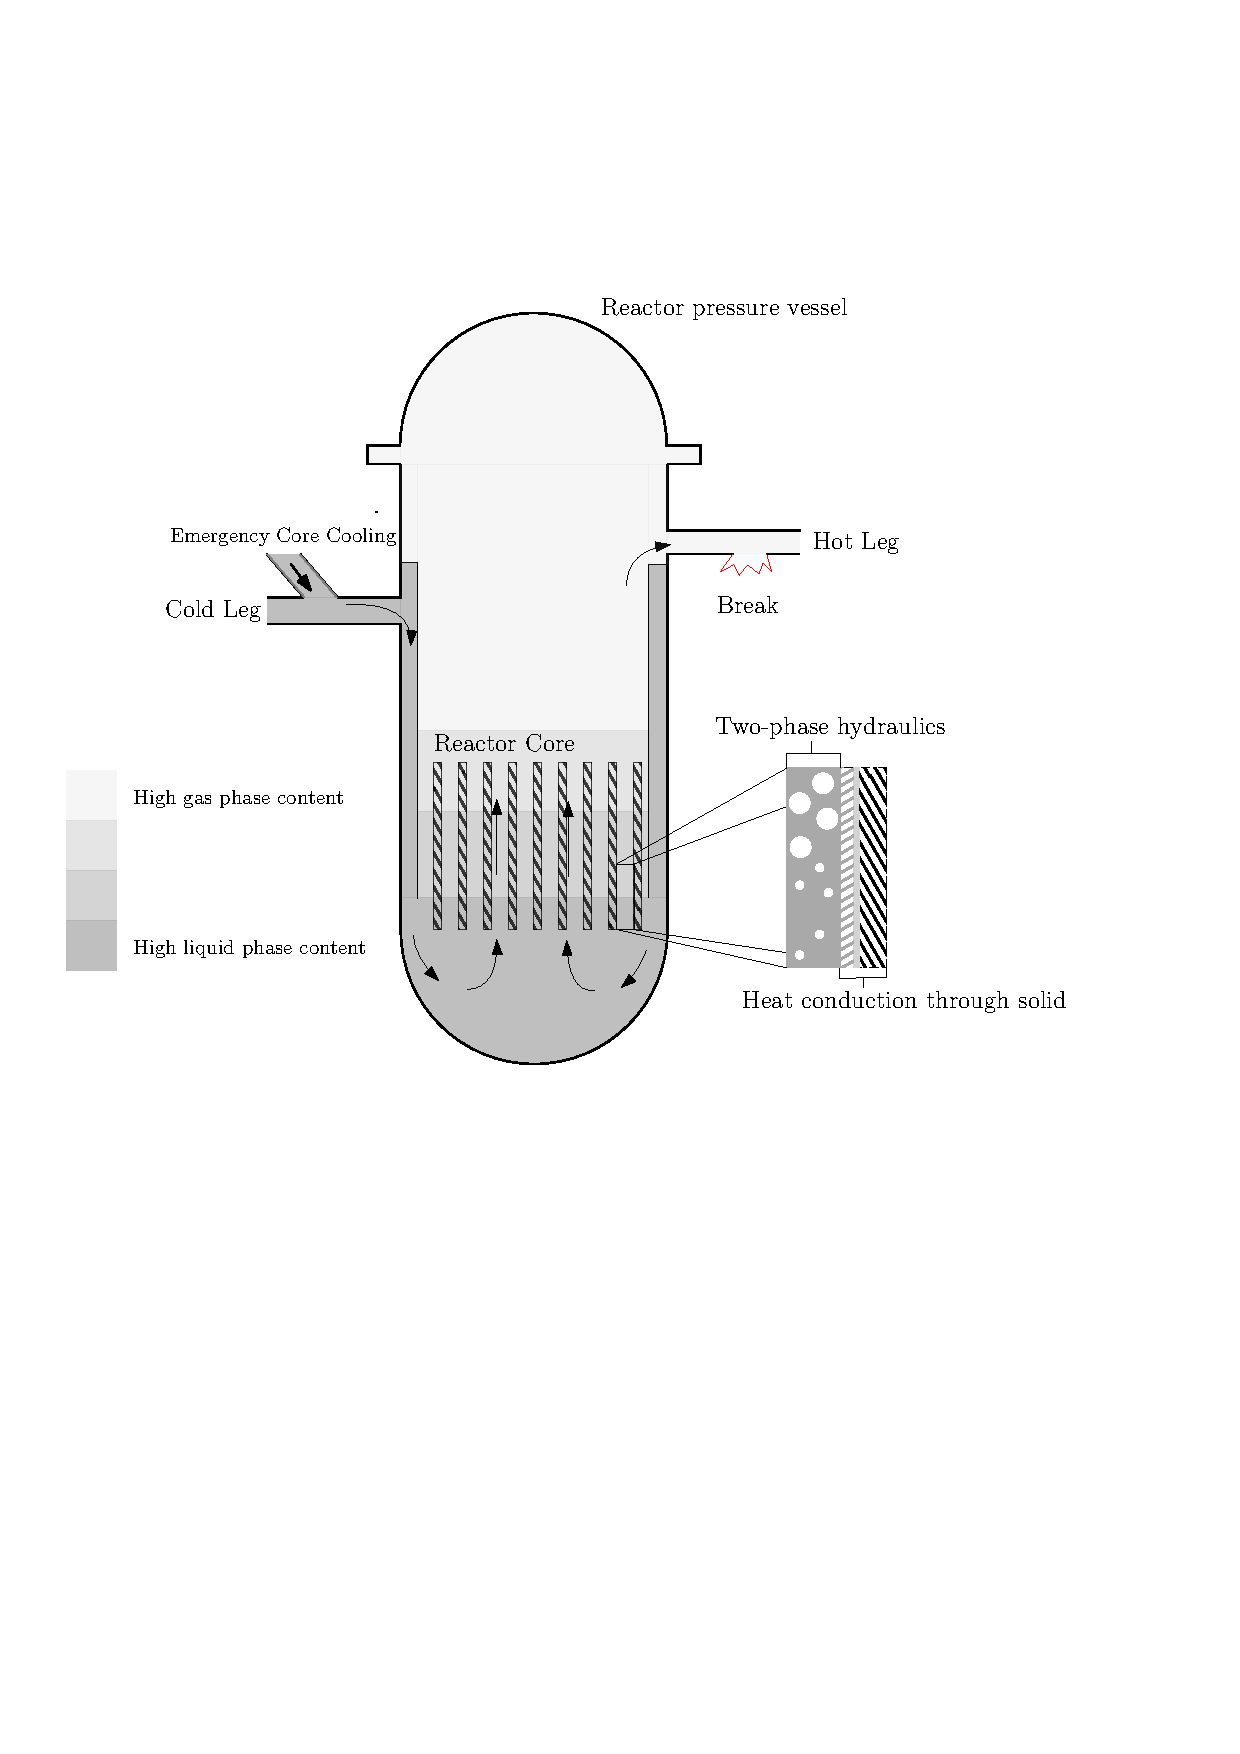
\includegraphics[scale=0.55]{../figures/heatedChannel/heatedChannel.pdf}
	\caption[Illustration of Heated Channel]{System thermal-hydraulics analysis encompasses many aspects of nuclear reactor system analysis, but the core of the problem for predicting the cladding temperature evolution (especially during accident condition) is to model properly and realistically the coolant flow in a heated channel in steady or transient condition. Here it is shown a simplified picture of loss of coolant accident in a \glsentryshort{pwr} where phase change along the heated channel occurs.}
	\label{fig:heated_channel}
\end{figure}

% Major difficulty
This remaining problem of modeling properly the two-phase flow in a heated channel, though much more limited in scope, is by no means trivial.
\marginpar{flow regimes}
This due to the fact that in two-phase flow, the morphological configurations of the flow (i.e., \emph{flow regimes}) can vary widely depending on many parameters such as difference in phase density, phasic velocity, and flow orientation.
Different morphological configuration implies different interfacial surface structure between the two phases (see Fig.~\ref{fig:flow_regimes}), 
which in turn affects the mass, momentum, and energy coupling terms (\emph{transfer relation}) between the phases.
At the same time, the interfacial surface and its deformation in an arbitrary flow configuration are not known \emph{a priori} and becomes part of the solution.
\begin{figure}[bth!]
	\centering
	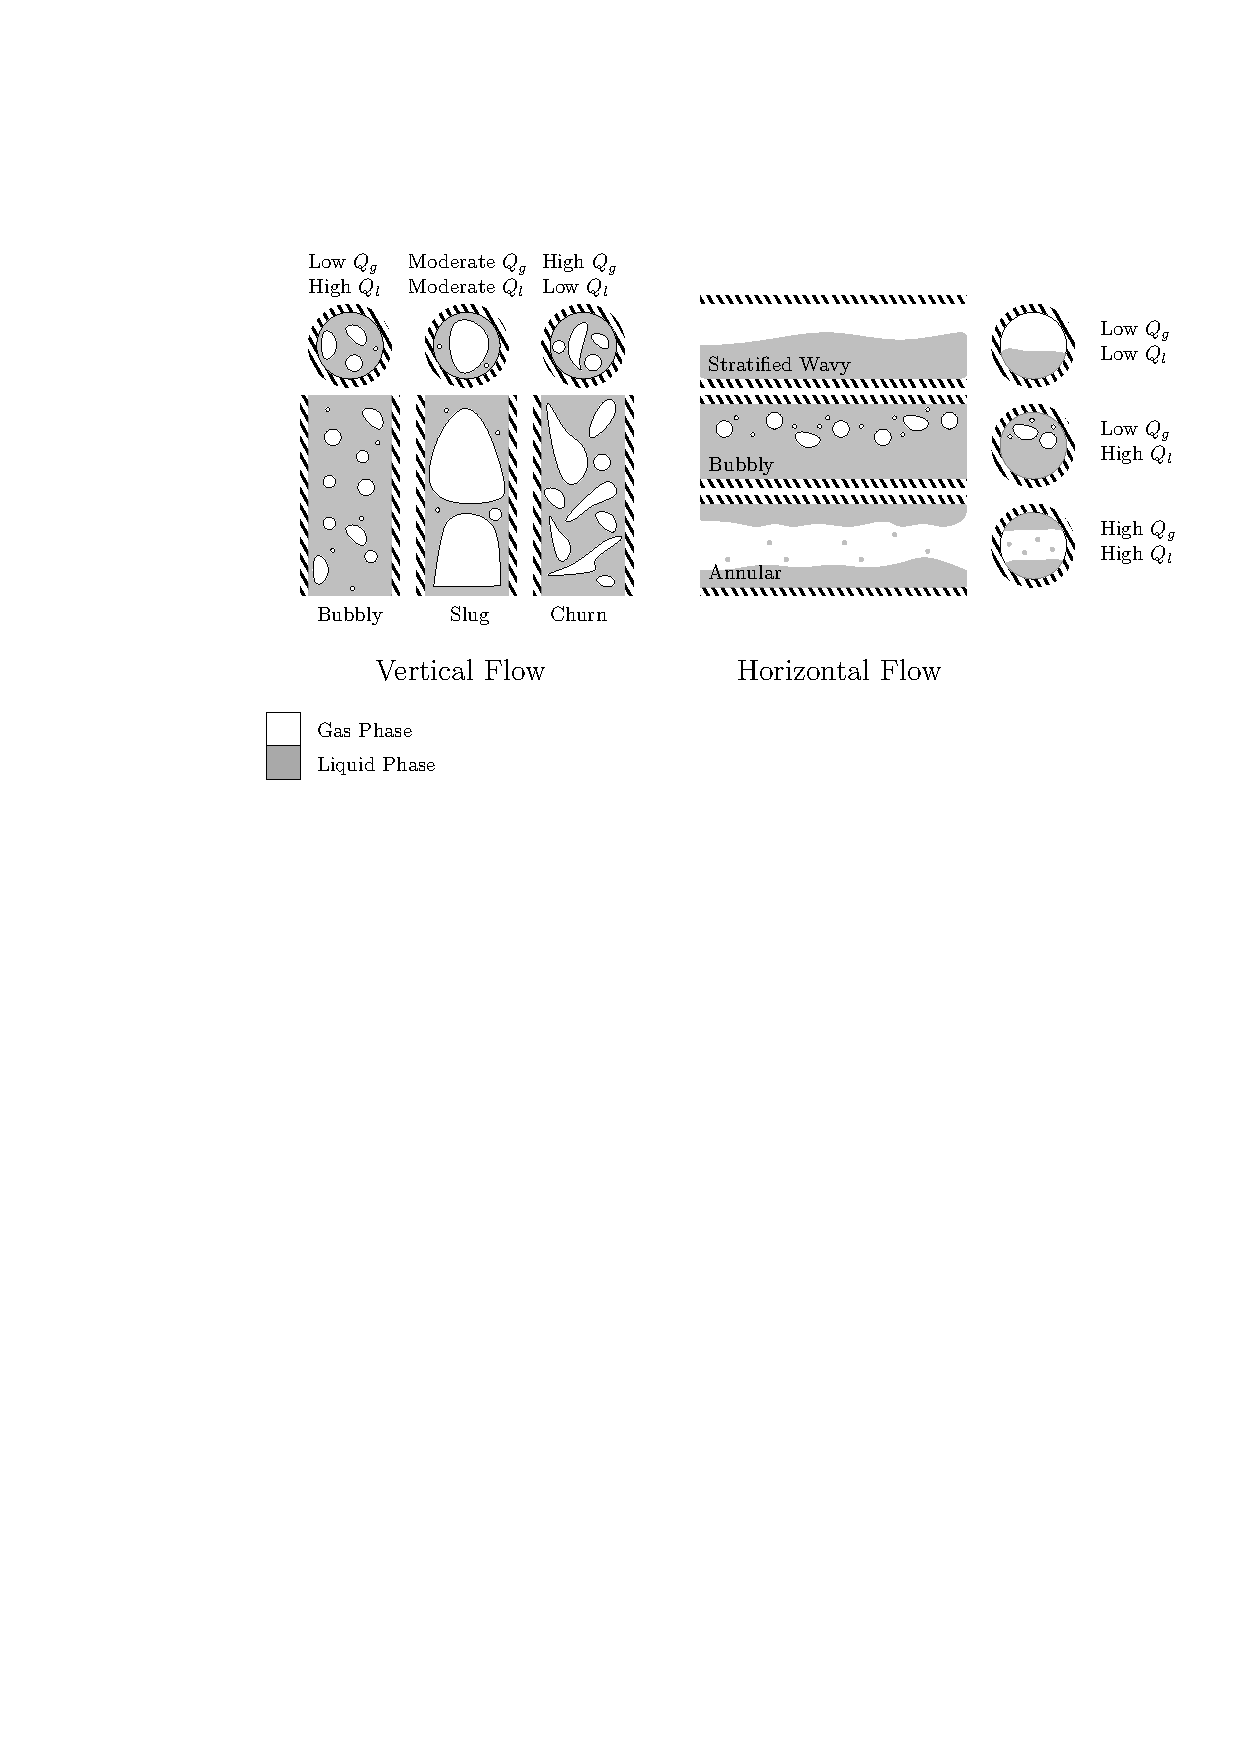
\includegraphics[width=\textwidth]{../figures/flowRegimes/flowRegimes.pdf}
	\caption[Some of the observed flow regimes in vertical and horizontal flow]{Some of the observed flow regimes in vertical and horizontal flow with different superficial liquid velocity, $Q_l = V_l / A$, and superficial gas velocity, $Q_g = V_g / A$, where $A$ is the flow area. The flows of both phases are co-current.}
	\label{fig:flow_regimes}
\end{figure}

% The rigorous approach, local instantaneous formulation
The most rigorous approach in describing two-phase flow is by using local instantaneous formulation where a set partial differential equations describing the conservation of mass, momentum, and energy, is formulated for each phase.
The two phases are, in turn, separated by zero-thickness interfacial surface.
The resulting set of equations fully describe the flow at any given location at any given time.
In addition to that, the solution of this formulation also respect the \emph{topological constraint} of the flow.
\marginpar{local instantaneous formulation, topological constraint}
The constraint states that only one phase can exist at any given time and at any given location in the flow \cite{Ghiaasiaan2007}.
This is illustrated in the Fig.~\ref{fig:phase_indicator_probe} where a hypothetical probe is put within a two-phase flow and a signal of indicator function $M(\mathbf{r}, t)$ is recorded.
\begin{figure}[bth!]
	\centering
	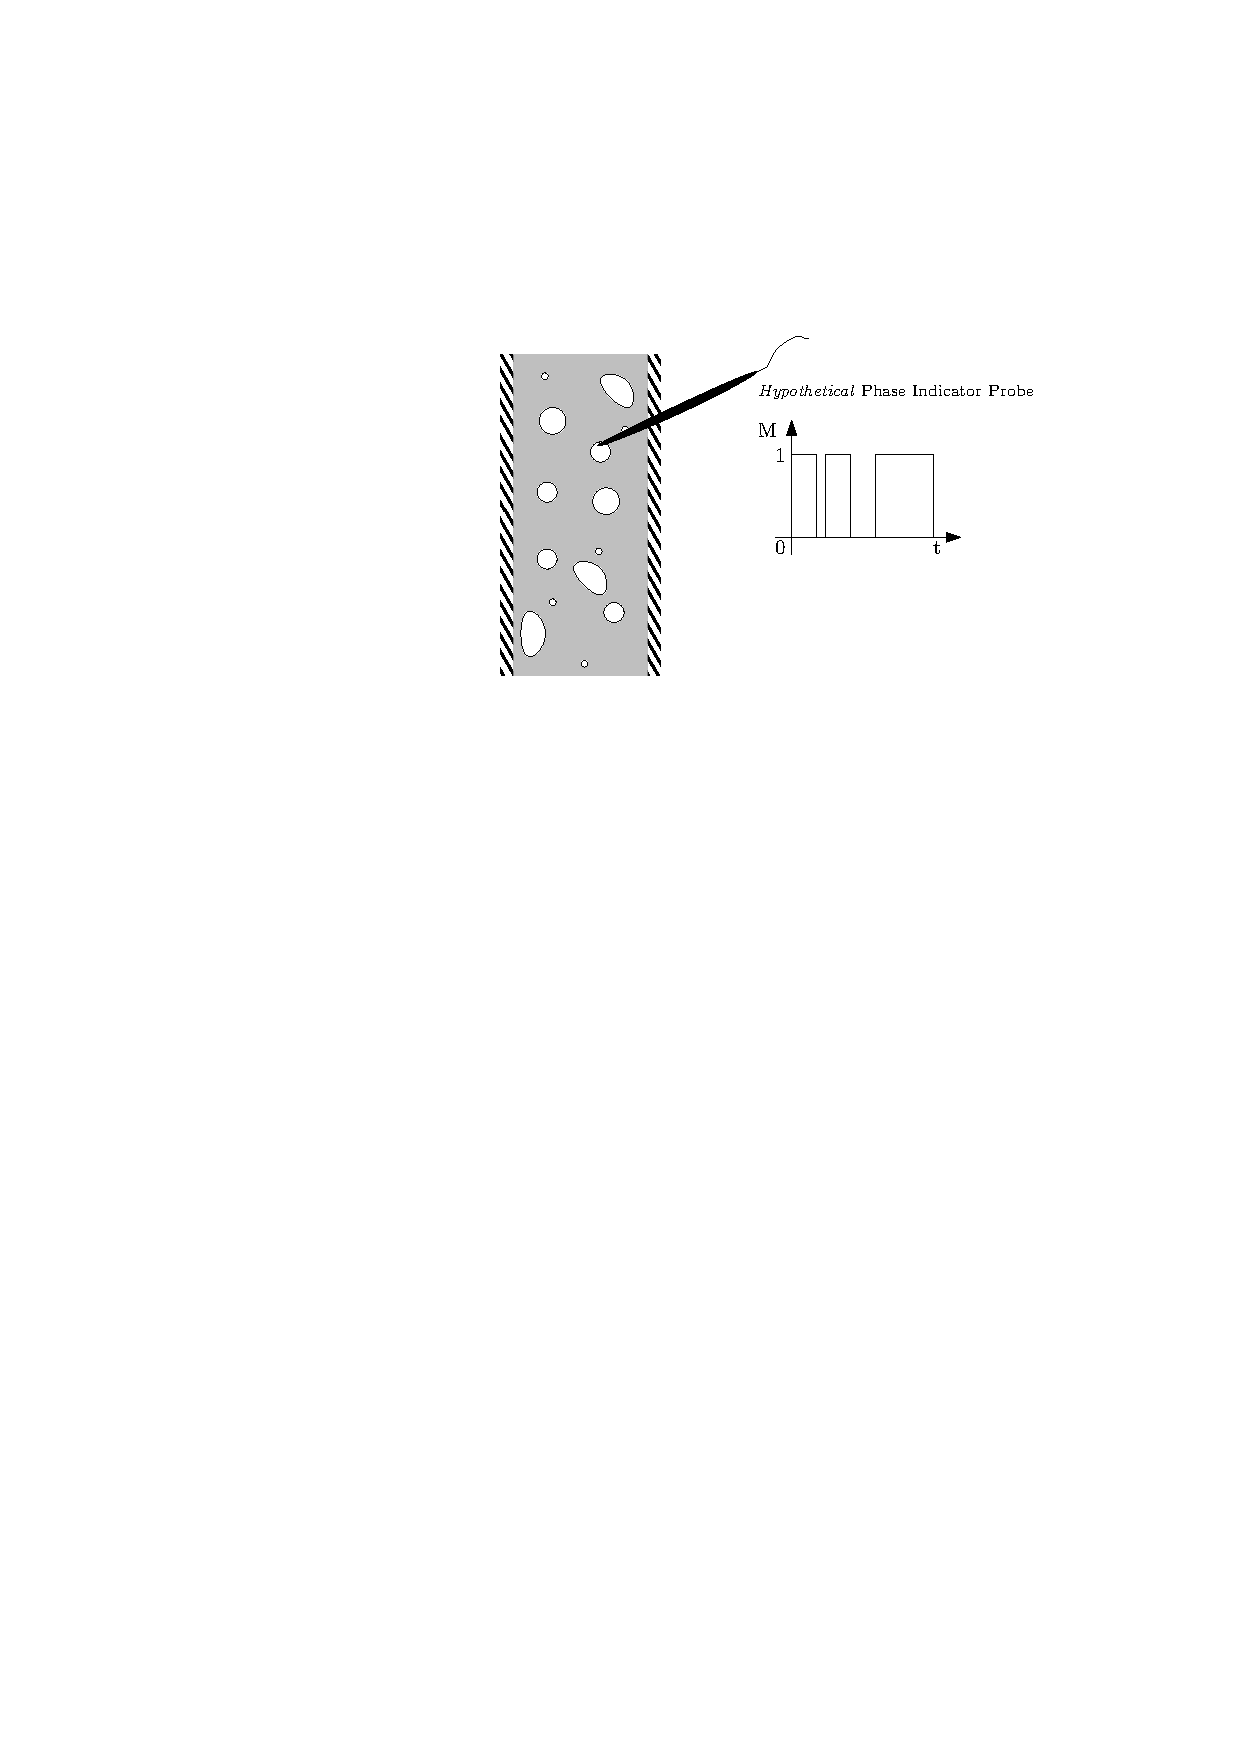
\includegraphics[scale=0.70]{../figures/phaseIndicatorProbe/phaseIndicatorProbe.pdf}
	\caption[A hypothetical phase indicator probe inside a channel of a two-phase flow]{Illustration of a hypothetical phase indicator probe inside a channel of a two-phase flow, recording at a point location the indicator function value (Eq.~(\ref{eq:indicator_function})) at every instance.}
	\label{fig:phase_indicator_probe}
\end{figure}
The indicator function is defined as,
\begin{equation}
  M (\mathbf{r}, t) =
    \begin{cases}
      1 \, ; \, \text{if probe tip in \text{gas phase}} \\
      0 \, ; \, \text{otherwise}
    \end{cases}
\label{eq:indicator_function}
\end{equation}
where \gls[hyper=false]{r} is vector of position;
and \gls[hyper=false]{t} is time.
The indicator function defined here is equivalent to the local instantaneous void fraction, 
which can be interpreted as the probability that the gas phase is present at a given point in space at a given moment \cite{USNRC2012}. 

As mentioned, the interfacial surface structure of the flow determines the coupling terms between the two phases.
\marginpar{resolving the motion of interfacial surface}
However, this surface and its deformation along the flow are not known \emph{a priori}.
As such, the solution of local instantaneous formulation of two-phase flow requires the motion of interfacial surface to be simultaneously resolved. 
As the time and length scales of the interfacial structure in a two-phase flow of an arbitrary morphological configurations can vary wildly,
the problem of resolving the motion of interfacial surface becomes intractable. 
Though advances have been made in the area of Computational Fluid Dynamics (CFD) in this regard, 
the problem remains intractable for the purpose of thermal-hydraulics system analysis (see \cite{Bestion2014} for recent review on the topic).

% The simplified approach, Time and Volume Averaged
To simplify the intractability problem of resolving the motion of interfacial surface motion in two-phase flow, 
time- and volume-average is carried out on the flow.
\marginpar{Time- and Volume-averaging}
Averaging can be seen as a filtering operation to remove the local temporal and spatial fluctuations (short scale variation) in the flow.
The length and duration which define short scale variation are problem specific 
(that is, at least qualitatively, not longer than the length and time scales of the flow configuration of interest).
The volume over which averaging is carried out is referred to either as a \emph{control volume}, a \emph{cell}, or a \emph{node}.

Averaging the indicator function both in time and in volume gives the void fraction,
\begin{equation}
  \langle \bar{\alpha} \rangle =  \frac{1}{\Delta V \Delta t} \int_{V}^{V + \Delta V} \int_{t}^{t + \Delta t} \alpha(\mathbf{r}, t) d\mathbf{r} dt = \frac{1}{\Delta V} \int_{V}^{V + \Delta V} \overline{\alpha(\mathbf{r})} d\mathbf{r}
\label{eq:void_fraction}
\end{equation}
Following the above formulation, void fraction can be interpreted as the fraction of the control volume occupied by the gas phase \cite{USNRC2012}. 
In the subsequent section the angle brackets and the overbar will be dropped from the void fraction notation 
and any mention of void fraction will refer to the time- and volume-averaged formulation given above.

% Two fluid model and its closure
Averaging the flow state variables in time and volume and using them to formulate a set of mass, momentum, and energy balance equations describing the fluid dynamics yield the so-called \emph{two-fluid model} \cite{Ishii2011}.
\marginpar{Time- and Volume-Averaged formulation, two-fluid model}
The model is the state of the art formulation for describing the dynamics of two-phase flow in system codes (which include, for example CATHARE, RELAP5, and \gls[hyper=false]{trace}).
This model separately treats the transport phenomena of the two phases of fluid resulting in six balance equations 
which are able to capture phenomena where thermal and mechanical non-equilibrium conditions exist between the two phases, conditions to be expected in wide range of \gls[hyper=false]{npp} transients.
\begin{figure}[bth]
	\centering
	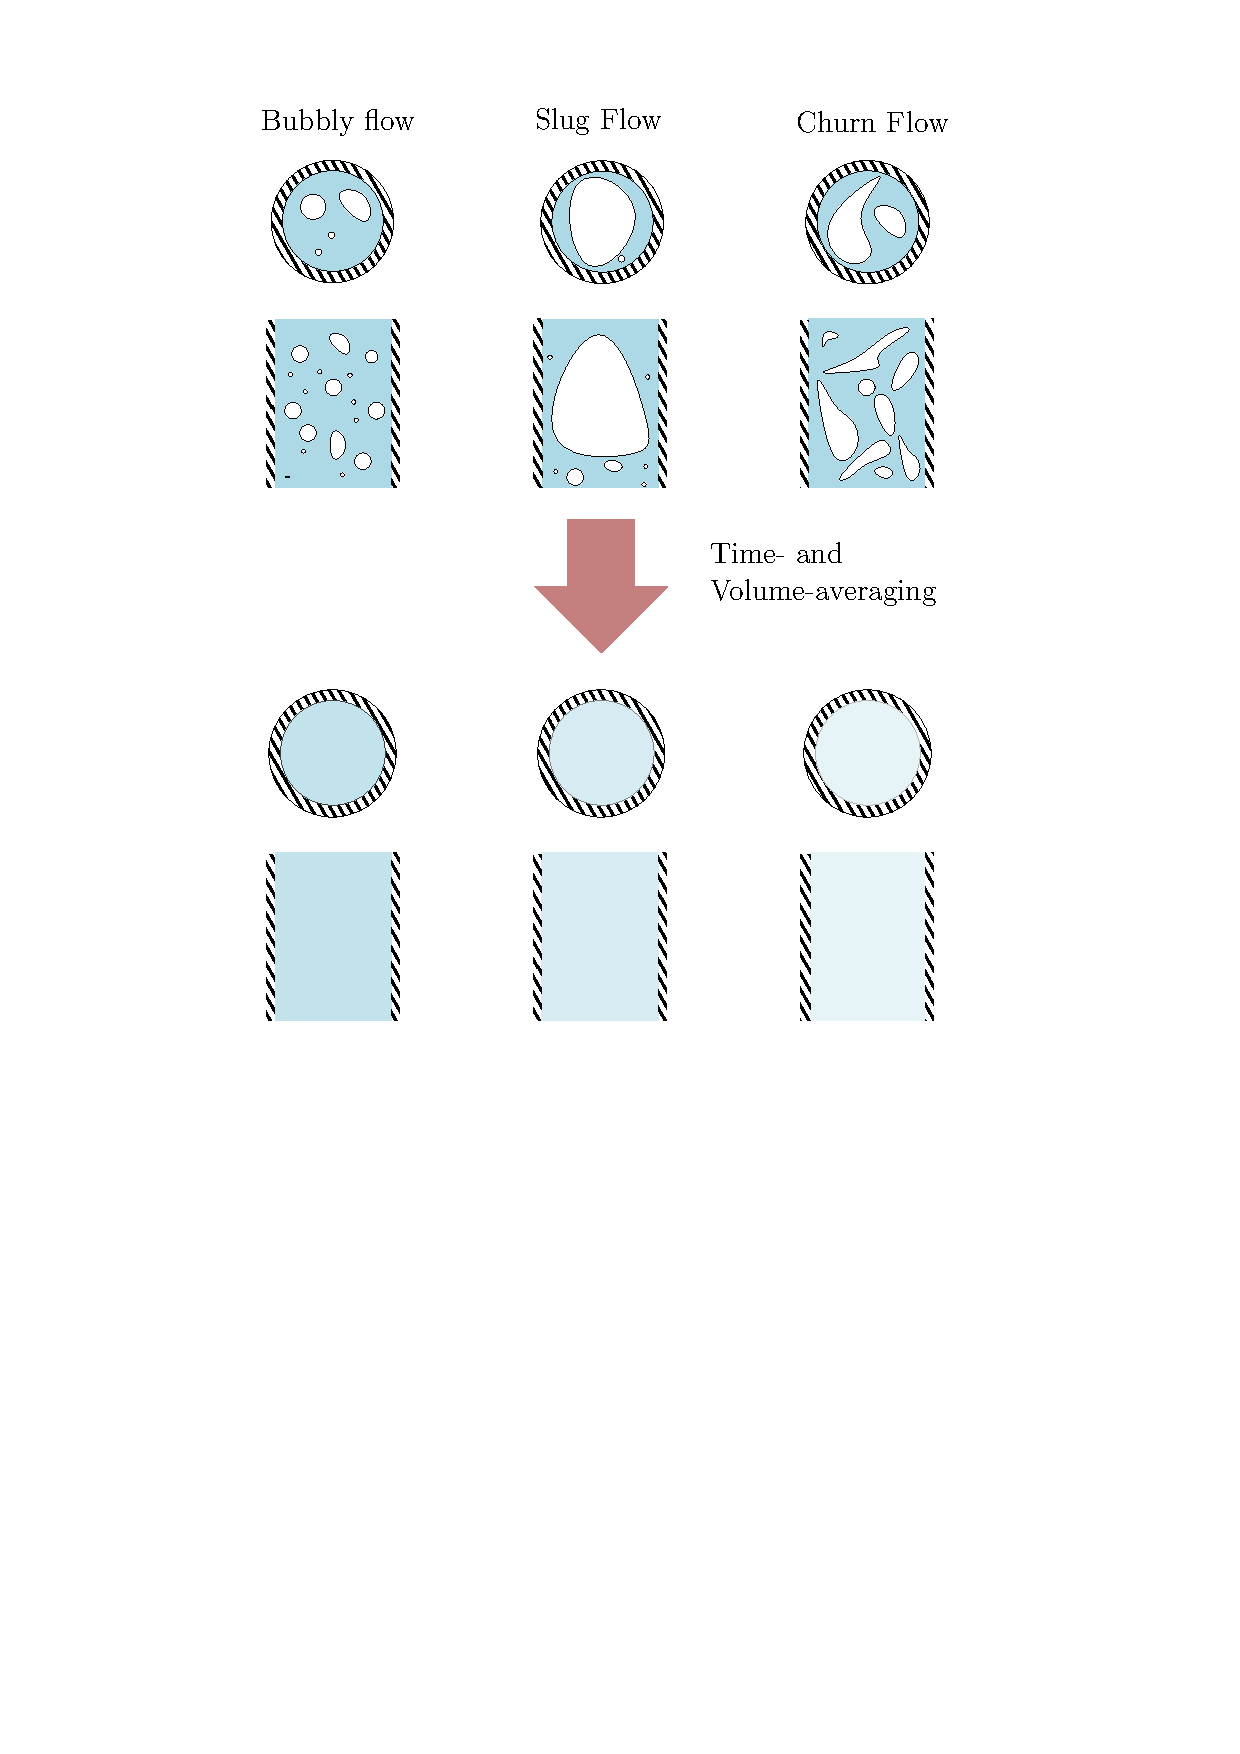
\includegraphics[scale=0.55]{../figures/flowAveraging/flowAveraging.pdf}
	\caption[Illustration of Flow Averaging]{Time and volume average carried out on the two-phase flow inside a channel results in a tractable form of fluid dynamics equation, but incur loss of information at the local level, especially when it comes to the interfacial structure between the two phases.}
	\label{fig:flow_averaging}
\end{figure}

% Closing paragraph
The next section will summarize the final formulation of the governing equations (time- and volume-averaged) adopted in \gls[hyper=false]{trace}, of which the complete derivation can be found in \cite{USNRC2012}.
As the averaging incurs loss of information regarding the flow local information (such as the interfacial structure between the phases, see Fig.~\ref{fig:flow_averaging}), 
the transfer relations between the two phases have to be recovered through the use of closure models briefly described in Section~\ref{sub:closure_and_flow_regimes}.
